\chapter{Nonlinear least squares on manifolds}
\label{ch:nls}

Chapter~\ref{ch:slam} turned SLAM into the minimisation of a sum of
squared, whitened residuals; Chapters~\ref{ch:rigid} and~\ref{ch:cameras}
gave us the residuals and their Jacobians. This chapter is about the
minimisation itself. Three algorithms cover almost everything a SLAM
back-end does: Gauss--Newton, which is fast when the model fits the data
well; Levenberg--Marquardt, which adds the safety net every practical
solver needs; and iteratively reweighted least squares, which makes both
robust to the wrong correspondences that grass will produce in large
numbers. All three work unchanged on manifolds once the vector-space
update $\x+\vect\delta$ is replaced by the retraction $\x\oplus
\vect\delta$ of Chapter~\ref{ch:rigid}. The practical finishes the camera
calibration started in Chapter~\ref{ch:cameras}.

\section{The problem}

\begin{definition}{Nonlinear least squares}{nls}
Given a twice continuously differentiable $\vect{r}:\R^n\to\R^m$,
$m\ge n$, minimise
\[
F(\x)=\tfrac12\norm{\vect{r}(\x)}^2=\tfrac12\sum_{i=1}^m r_i(\x)^2 .
\]
We write $J(\x)=\partial\vect{r}/\partial\x\in\R^{m\times n}$,
$\vect{g}=J\T\vect{r}$ and $H=J\T J$.
\end{definition}

The residuals are always the whitened ones of Chapter~\ref{ch:slam}, so
every $r_i$ is measured in standard deviations and the scale of $F$ has
a statistical meaning, which we exploit at the end of the chapter.

\begin{proposition}{Gradient and Hessian}{gradhess}
$\nabla F=J\T\vect{r}=\vect{g}$ and
$\nabla^2F=J\T J+S$ with $S=\sum_{i=1}^m r_i\,\nabla^2r_i$.
\end{proposition}

\begin{proof}
$\partial F/\partial x_k=\sum_ir_i\,\partial r_i/\partial x_k=(J\T
\vect{r})_k$. Differentiating once more,
$\partial^2F/\partial x_k\partial x_l=\sum_i\bigl(\partial_kr_i\,
\partial_lr_i+r_i\,\partial_k\partial_lr_i\bigr)$, which is
$(J\T J)_{kl}+S_{kl}$.
\end{proof}

\begin{inwords}
The Hessian has a part that only needs first derivatives, $J\T J$, and a
part $S$ that needs second derivatives but is multiplied by the residuals
themselves. When the model explains the data well, the residuals are
small and so is $S$. Every method of this chapter bets on that.
\end{inwords}

\section{Gauss--Newton}

Linearise the residual around the current estimate,
$\vect{r}(\x+\vect\delta)\approx\vect{r}+J\vect\delta$, and minimise the
resulting quadratic model
\begin{equation}\label{eq:model}
L(\vect\delta)=\tfrac12\norm{\vect{r}+J\vect\delta}^2
=F+\vect\delta\T\vect{g}+\tfrac12\vect\delta\T H\vect\delta .
\end{equation}
When $J$ has full column rank, $H\succ0$, $L$ is strictly convex and its
minimiser solves the \emph{normal equations}
\begin{equation}\label{eq:gn}
H\,\vect\delta_{\mathrm{gn}}=-\vect{g}.
\end{equation}
Gauss--Newton iterates $\x\leftarrow\x+\vect\delta_{\mathrm{gn}}$. It is
Newton's method with $S$ dropped from the Hessian.

\begin{theorem}{Local behaviour of Gauss--Newton}{gnrate}
Let $\x^\star$ be a stationary point of $F$ with $H(\x^\star)\succ0$,
and $\varphi(\x)=\x-H(\x)^{-1}\vect{g}(\x)$ the Gauss--Newton map. Then
$\varphi(\x^\star)=\x^\star$ and
\[
D\varphi(\x^\star)=-H(\x^\star)^{-1}S(\x^\star).
\]
The eigenvalues of this matrix are real. If its spectral radius
$\varrho$ is below $1$, Gauss--Newton converges to $\x^\star$ from every
starting point close enough, linearly with any rate above $\varrho$; if
$\vect{r}(\x^\star)=\vect0$ then $S(\x^\star)=0$ and the convergence is
superlinear. If $\varrho>1$, $\x^\star$ repels the iteration along the
corresponding eigenvector.
\end{theorem}

\begin{proof}
$\vect{g}(\x^\star)=\vect0$, so $\varphi(\x^\star)=\x^\star$. Near
$\x^\star$, $H(\x)$ is invertible and continuous, and
$\vect{g}(\x)=\nabla^2F(\x^\star)(\x-\x^\star)+o(\norm{\x-\x^\star})$.
Hence
\begin{align*}
\varphi(\x)-\x^\star
&=(\x-\x^\star)-\bigl(H(\x^\star)^{-1}+o(1)\bigr)\bigl(\nabla^2F(\x^\star)
 (\x-\x^\star)+o(\norm{\x-\x^\star})\bigr)\\
&=\bigl(I-H(\x^\star)^{-1}(H(\x^\star)+S(\x^\star))\bigr)(\x-\x^\star)
 +o(\norm{\x-\x^\star})\\
&=-H(\x^\star)^{-1}S(\x^\star)(\x-\x^\star)+o(\norm{\x-\x^\star}),
\end{align*}
which is the derivative. $H^{-1}S$ is similar to the symmetric matrix
$H^{-1/2}SH^{-1/2}$, so its eigenvalues are real. The convergence
statements are Ostrowski's theorem on fixed-point iterations: an
iteration whose derivative at a fixed point has spectral radius
$\varrho<1$ converges locally with every linear rate above $\varrho$,
and superlinearly when $\varrho=0$; a fixed point with an eigenvalue of
modulus above $1$ is not attracting in that direction.
\end{proof}

\begin{example}{When Gauss--Newton fails}{mnt}
Take $n=1$ and $\vect{r}(x)=(x+1,\ \lambda x^2+x-1)$ (Madsen, Nielsen
and Tingleff). Then $x^\star=0$ is stationary, $F(0)=1$ (a
\emph{large}-residual problem), $H(0)=1+1=2$ and
$S(0)=r_2(0)\,r_2''(0)=-2\lambda$, so by \cref{thm:gnrate} the
Gauss--Newton error is multiplied by $\lambda$ at each step. Moreover
$F''(0)=H+S=2-2\lambda$, so $x^\star=0$ is a strict minimum for every
$\lambda<1$. For $\lambda=-2$ it is a perfectly good minimum, and
Gauss--Newton is repelled from it, oscillating with growing amplitude;
\cref{fig:gnrate} shows it, together with Levenberg--Marquardt
converging on the same problem.
\end{example}

\begin{figure}[ht]
\centering
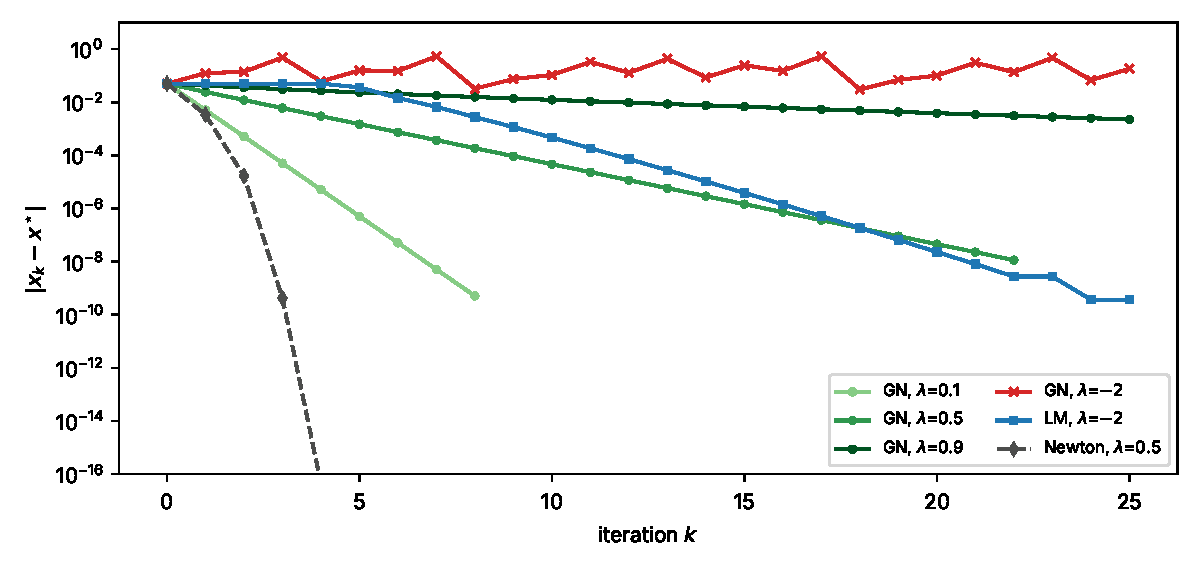
\includegraphics[width=0.85\linewidth]{figures/ch04_gn_rate.pdf}
\caption{Error per iteration on \cref{ex:mnt}. Gauss--Newton converges
linearly with ratio $\lambda$, fails for $\lambda=-2$, and is beaten by
Newton's method with the exact Hessian (quadratic convergence).
Levenberg--Marquardt converges for $\lambda=-2$.}
\label{fig:gnrate}
\end{figure}

\begin{lemma}{Descent and conditioning}{gndescent}
If $\vect{g}\neq\vect0$ and $H\succ0$, the Gauss--Newton step is a
descent direction: $\vect{g}\T\vect\delta_{\mathrm{gn}}<0$. The
condition number of the normal equations is the square of that of the
Jacobian: $\kappa_2(J\T J)=\kappa_2(J)^2$.
\end{lemma}

\begin{proof}
$\vect{g}\T\vect\delta_{\mathrm{gn}}=-\vect{g}\T H^{-1}\vect{g}<0$ since
$H^{-1}\succ0$. If $J=U\Sigma V\T$ is a thin SVD, $J\T J=V\Sigma^2V\T$,
whose singular values are the $\sigma_i^2$; the condition number is the
ratio of the largest to the smallest.
\end{proof}

A descent direction is not a descent \emph{step}: nothing guarantees that
$F(\x+\vect\delta_{\mathrm{gn}})<F(\x)$, and in the calibration below the
very first Gauss--Newton step multiplies the cost by twenty before the
method recovers (\cref{fig:calib}). The squared condition number is why
dense solvers prefer a QR factorisation of $J$ to a Cholesky
factorisation of $J\T J$; SLAM back-ends nevertheless form the normal
equations, because their sparsity (\cref{prop:sparsity}) is what makes
large problems tractable (Chapter~8).

\section{Levenberg--Marquardt}

\begin{definition}{Levenberg--Marquardt step}{lm}
For a damping $\lambda>0$ and a positive diagonal matrix $D$, the
Levenberg--Marquardt step solves
\begin{equation}\label{eq:lm}
(H+\lambda D)\,\vect\delta=-\vect{g}.
\end{equation}
Levenberg used $D=I$; Marquardt's choice $D=\diag(H)$ makes the method
invariant to rescaling individual parameters.
\end{definition}

\begin{proposition}{Properties of the damped step}{lmprops}
Let $\vect\delta(\lambda)$ solve \eqref{eq:lm}.
\begin{enumerate}[label=(\roman*),nosep]
\item $H+\lambda D\succ0$, so $\vect\delta(\lambda)$ is unique, and it is
  a descent direction whenever $\vect{g}\neq\vect0$, even if $J$ is rank
  deficient.
\item As $\lambda\to0$, $\vect\delta(\lambda)\to\vect\delta_{\mathrm{gn}}$
  (when $H\succ0$); as $\lambda\to\infty$,
  $\lambda\vect\delta(\lambda)\to-D^{-1}\vect{g}$, a short step along the
  scaled steepest-descent direction.
\item (Trust region; $D=I$.) $\vect\delta(\lambda)$ minimises the model
  $L$ of \eqref{eq:model} over the ball $\norm{\vect\delta}\le\Delta$
  with $\Delta=\norm{\vect\delta(\lambda)}$, and
  $\lambda\mapsto\norm{\vect\delta(\lambda)}$ is decreasing.
\end{enumerate}
\end{proposition}

\begin{proof}
(i) $H\succeq0$ and $\lambda D\succ0$. Descent:
$\vect{g}\T\vect\delta=-\vect{g}\T(H+\lambda D)^{-1}\vect{g}<0$.
(ii) The first limit is continuity of the inverse. For the second,
$\lambda\vect\delta=-(H/\lambda+D)^{-1}\vect{g}\to-D^{-1}\vect{g}$.
(iii) $\vect\delta=\vect\delta(\lambda)$ is the unique minimiser of the
strictly convex function $L(\vect\delta')+\frac\lambda2\norm{\vect
\delta'}^2$, whose gradient $\vect{g}+H\vect\delta'+\lambda\vect\delta'$
vanishes at $\vect\delta$. Hence for any $\vect\delta'$ with
$\norm{\vect\delta'}\le\Delta$,
\[
L(\vect\delta')\ge L(\vect\delta)+\tfrac\lambda2\bigl(\norm{\vect
\delta}^2-\norm{\vect\delta'}^2\bigr)\ge L(\vect\delta).
\]
For the monotonicity, write $H=Q\Lambda Q\T$ with eigenvalues
$\lambda_i\ge0$; then $\norm{\vect\delta(\lambda)}^2=\sum_i(\vect{q}_i\T
\vect{g})^2/(\lambda_i+\lambda)^2$, a decreasing function of $\lambda$.
\end{proof}

\begin{inwords}
The damping is a dial between two methods. Turned down, LM is
Gauss--Newton and inherits its speed near a good solution; turned up, it
takes small, safe gradient steps. Equivalently, $\lambda$ sets the radius
of the region in which we trust the linearisation. All that remains is
to turn the dial automatically, by comparing what the model promised with
what the true cost delivered.
\end{inwords}

\begin{lemma}{Predicted decrease}{gain}
For the step of \eqref{eq:lm}, the decrease predicted by the model is
\[
L(\vect0)-L(\vect\delta)=\tfrac12\,\vect\delta\T\bigl(\lambda D\vect\delta
-\vect{g}\bigr)>0 .
\]
\end{lemma}

\begin{proof}
From \eqref{eq:model}, $L(\vect0)-L(\vect\delta)=-\vect\delta\T\vect{g}-
\tfrac12\vect\delta\T H\vect\delta$, and \eqref{eq:lm} gives
$H\vect\delta=-\vect{g}-\lambda D\vect\delta$. Substituting,
$-\vect\delta\T\vect{g}+\tfrac12\vect\delta\T\vect{g}+\tfrac\lambda2
\vect\delta\T D\vect\delta=\tfrac12\vect\delta\T(\lambda D\vect\delta-
\vect{g})$. Both terms are positive: $\vect\delta\T D\vect\delta>0$ and
$-\vect\delta\T\vect{g}>0$ by \cref{prop:lmprops}(i).
\end{proof}

The \emph{gain ratio}
$\varrho=\bigl(F(\x)-F(\x+\vect\delta)\bigr)/\bigl(L(\vect0)-L(\vect
\delta)\bigr)$ compares the actual and the predicted decrease. The step
is accepted if $\varrho>0$. Nielsen's rule then updates the damping
smoothly: on acceptance, $\lambda\leftarrow\lambda\max\{\tfrac13,\,1-
(2\varrho-1)^3\}$ and $\nu\leftarrow2$; on rejection,
$\lambda\leftarrow\nu\lambda$ and $\nu\leftarrow2\nu$. A ratio near 1
means the model is good and the damping can drop; a negative ratio
means the step was too ambitious and is retried with more damping. This
is the algorithm in \code{optim.levenberg\_marquardt}, and in substance
the one inside Ceres, g2o and GTSAM (which also offer Powell's dog-leg, a
different way of searching the same trust region).

\section{Robust kernels}

A single wrong correspondence with a residual of 100 standard deviations
contributes $5000$ to $F$, more than a thousand correct ones, and drags
the solution towards itself. On a lawn, where feature matching produces
many such errors, plain least squares is useless (\cref{fig:robust}).

\begin{definition}{Robust cost}{robust}
Partition the residuals into blocks $\vect{r}_i\in\R^{m_i}$ (one per
measurement, e.g.\ a pixel) and let $s_i=\norm{\vect{r}_i}^2$. A
\emph{kernel} is a $C^1$ function $\rho:[0,\infty)\to[0,\infty)$ with
$\rho(0)=0$, $\rho'(0)=1$ and $\rho'>0$ nonincreasing; the robust cost is
$F_\rho=\tfrac12\sum_i\rho(s_i)$. With a threshold $k>0$:
\begin{align*}
\text{Huber:}&\quad\rho(s)=s\ \ (s\le k^2),\qquad 2k\sqrt{s}-k^2\ \
(s>k^2);\\
\text{Cauchy:}&\quad\rho(s)=k^2\log\bigl(1+s/k^2\bigr).
\end{align*}
$\rho(s)=s$ recovers plain least squares.
\end{definition}

\begin{proposition}{Iteratively reweighted least squares}{irls}
$\nabla F_\rho=\sum_iw_i\,J_i\T\vect{r}_i$ with $w_i=\rho'(s_i)$ and
$J_i=\partial\vect{r}_i/\partial\x$. Consequently $\x^\star$ is a
stationary point of $F_\rho$ if and only if it is a stationary point of
the weighted least-squares cost $\tfrac12\sum_iw_i\norm{\vect{r}_i}^2$
with the weights frozen at their values at $\x^\star$.
\end{proposition}

\begin{proof}
By the chain rule,
$\nabla\bigl(\tfrac12\rho(\vect{r}_i\T\vect{r}_i)\bigr)=\tfrac12\rho'(
s_i)\cdot2J_i\T\vect{r}_i$. With frozen weights the gradient of the
weighted cost is $\sum_iw_iJ_i\T\vect{r}_i$, the same vector at
$\x^\star$.
\end{proof}

So a robust problem is solved by any of the previous methods applied to
the residuals $\sqrt{w_i}\,\vect{r}_i$ and Jacobians $\sqrt{w_i}\,J_i$,
with the weights recomputed at every iteration; the cost used to accept
or reject steps is $F_\rho$ itself. This is what the solvers in
\code{vslam.optim} do when given a \code{kernel}. (Triggs et al.\ add a
second-order correction involving $\rho''$; for the redescending kernels
used in practice it changes little.)

\begin{inwords}
The weight $w=\rho'(s)$ says how much a residual is believed. Least
squares believes everything equally. Huber believes residuals up to $k$
standard deviations fully and gives larger ones a weight $k/\norm{
\vect{r}}$: their \emph{influence} on the gradient, weight times
residual, is capped at $k$. Cauchy goes further: its influence decreases
back to zero for large residuals, so gross outliers are effectively
ignored (\cref{fig:robust}, left). The price is that the Cauchy cost is
not convex (Exercise~\ref{ex:4cauchy}), so it needs a decent starting
point --- in Chapter~7 that will come from RANSAC.
\end{inwords}

\begin{figure}[ht]
\centering
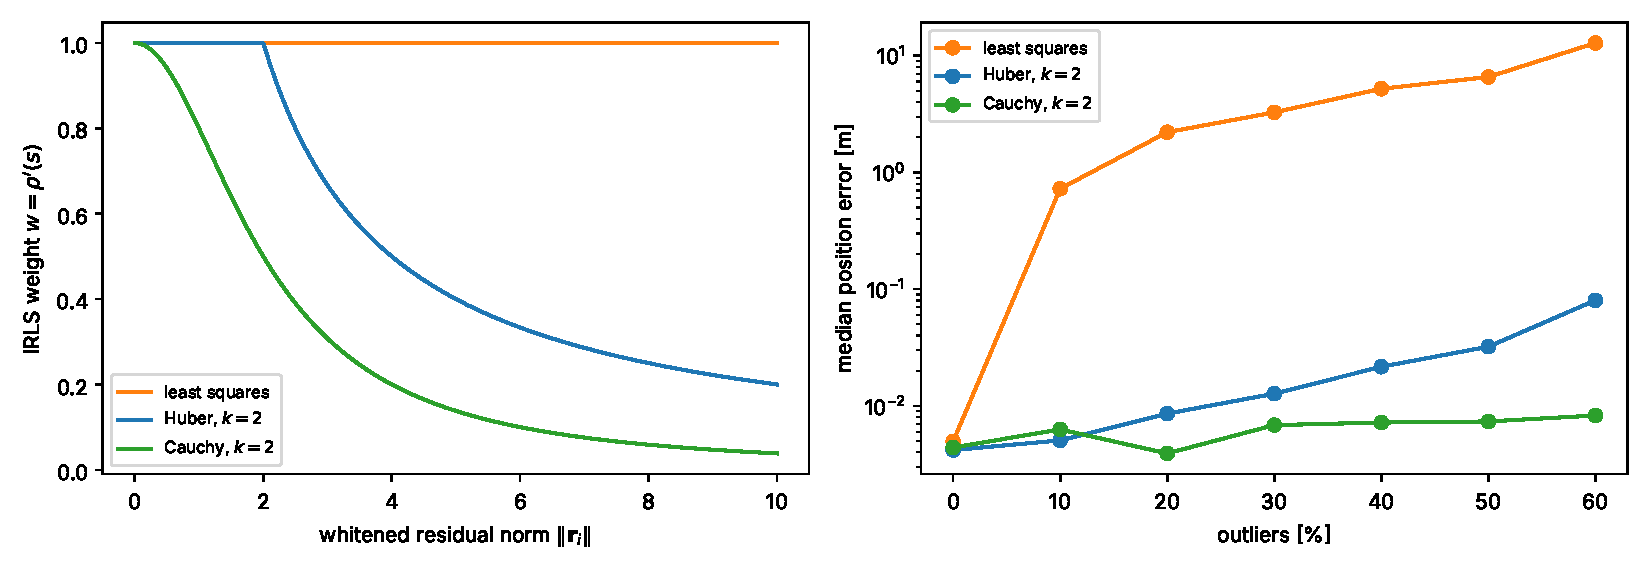
\includegraphics[width=\linewidth]{figures/ch04_robust.pdf}
\caption{Left: IRLS weights of three kernels as a function of the
whitened residual norm. Right: median position error of a camera pose
refined from 100 correspondences, a growing fraction of which are random
pixels (20 trials per point, LM from a perturbed start). Least squares
breaks at the first outlier; Huber degrades gracefully; Cauchy is
unaffected up to 60\,\% outliers.}
\label{fig:robust}
\end{figure}

\section{On manifolds}

Nothing above used the vector-space structure of $\R^n$ except in the
update $\x+\vect\delta$. Replace it by a retraction.

\begin{definition}{Least squares on a manifold}{nlsman}
Let the unknown $\x$ live in a product of vector spaces and Lie groups,
with the plus operator $\x\oplus\vect\delta$ of \cref{def:plusminus}
acting componentwise. At the current estimate $\x$, define
$\tilde{\vect{r}}(\vect\delta)=\vect{r}(\x\oplus\vect\delta)$ and its
Jacobian $J=\partial\tilde{\vect{r}}/\partial\vect\delta$ at
$\vect\delta=\vect0$ (the right Jacobians of Chapter~\ref{ch:rigid}).
One iteration of Gauss--Newton or LM computes $\vect\delta$ from $J$ and
$\tilde{\vect{r}}(\vect0)$ exactly as before, then sets
$\x\leftarrow\x\oplus\vect\delta$.
\end{definition}

Each iteration therefore solves an ordinary problem in a local chart
centred on the current estimate. Since $\vect\delta\mapsto\x\oplus
\vect\delta$ is a diffeomorphism from a neighbourhood of $\vect0$ onto a
neighbourhood of $\x$ (the exponential map is a local diffeomorphism),
$\x^\star$ is a local minimiser of $F$ on the manifold exactly when
$\vect0$ is a local minimiser of $\vect\delta\mapsto F(\x^\star\oplus
\vect\delta)$; stationarity means $J\T\vect{r}=\vect0$ in that chart.
Re-centring the chart at every iteration keeps $\vect\delta$ small, so
the singularities of any global parametrisation are never met. The
code needs nothing more than a \code{retract} method: the notebook
optimises a rotation this way and recovers the closed-form solution of
\cref{lem:nearestrot}.

\begin{proposition}{Uncertainty at the optimum}{laplace}
Assume the residuals are whitened Gaussian measurement errors, so that
the posterior is proportional to $e^{-F}$, and let $\x^\star$ be the
minimiser with $H=J\T J\succ0$ at $\x^\star$.
\begin{enumerate}[label=(\roman*),nosep]
\item (Laplace approximation.) Neglecting $S$ and terms of order three,
  $\x=\x^\star\oplus\vect\delta$ with $\vect\delta\sim\Normal(\vect0,
  H^{-1})$.
\item (Consistency check.) For a linear model $\vect{r}(\x)=A\x-\vect{b}$
  with $\vect{b}=A\x_0+\vect\epsilon$, $\vect\epsilon\sim\Normal(\vect0,
  I_m)$ and $A$ of rank $n$, one has $\E[2F(\x^\star)]=m-n$.
\end{enumerate}
\end{proposition}

\begin{proof}
(i) Expand $\vect\delta\mapsto F(\x^\star\oplus\vect\delta)$ to second
order at $\vect0$: the gradient vanishes and the Hessian is $H+S$
(\cref{prop:gradhess}); with $S$ neglected,
$e^{-F(\x^\star\oplus\vect\delta)}\propto e^{-\frac12\vect\delta\T
H\vect\delta}$, the density of $\Normal(\vect0,H^{-1})$.
(ii) $\x^\star=(A\T A)^{-1}A\T\vect{b}$, so the residual at the optimum
is $\vect{r}^\star=-(I-\Pi)\vect{b}=-(I-\Pi)\vect\epsilon$ with
$\Pi=A(A\T A)^{-1}A\T$ the orthogonal projector onto the range of $A$
($(I-\Pi)A\x_0=\vect0$). $I-\Pi$ is an orthogonal projector of rank
$m-n$, so $\E\norm{\vect{r}^\star}^2=\E[\vect\epsilon\T(I-\Pi)
\vect\epsilon]=\tr(I-\Pi)=m-n$.
\end{proof}

\begin{inwords}
The matrix we already factorise to compute the step is, inverted, the
covariance of the answer. And the final cost tells us whether to believe
it: with whitened residuals, $F$ should end near $\tfrac12(m-n)$. A much
larger value means the noise model is too optimistic or the model is
wrong; that is the first number to look at when a calibration or a SLAM
run misbehaves. With a gauge freedom (Chapter~\ref{ch:slam}) $H$ is
singular, and the covariance only makes sense after the gauge is fixed.
\end{inwords}

\section{Practice: finishing the calibration}

The calibration problem of Chapter~\ref{ch:cameras} has the state
\[
\x=(\vect\kappa,\,T_{bc_1},\dots,T_{bc_N}),\qquad
\vect\kappa=(f_x,f_y,c_x,c_y,k_1,k_2,p_1,p_2,k_3),
\]
with one camera pose per view, and one whitened residual per corner and
view, $\vect{e}_{ij}=\bigl(\z_{ij}-\vect{u}(\vect\kappa,T_{bc_i},\p_j)
\bigr)/\sigma$. The pose Jacobian is \cref{prop:projjac}; the intrinsic
one follows from \cref{def:distortion}:
\begin{gather*}
\frac{\partial\vect{u}}{\partial(f_x,f_y,c_x,c_y)}=\begin{pmatrix}x_d&0&1
&0\\0&y_d&0&1\end{pmatrix},\\
\frac{\partial\vect{u}}{\partial(k_1,k_2,p_1,p_2,k_3)}=F\begin{pmatrix}
xr^2&xr^4&2xy&r^2+2x^2&xr^6\\yr^2&yr^4&r^2+2y^2&2xy&yr^6\end{pmatrix}.
\end{gather*}
Zhang's linear step initialises $K$ and the poses, the distortion starts
at zero, and LM (or Gauss--Newton) does the rest.

\begin{figure}[ht]
\centering
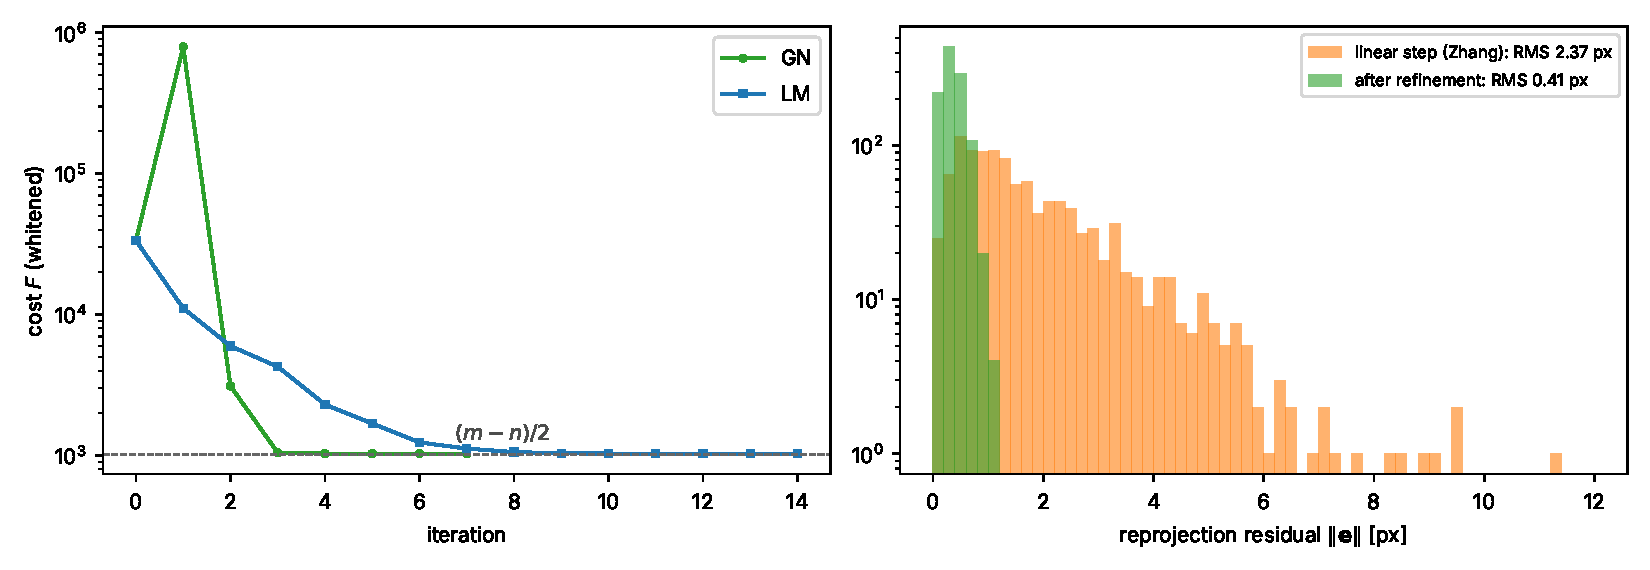
\includegraphics[width=\linewidth]{figures/ch04_calibration.pdf}
\caption{Calibration of the wide-angle camera of \cref{fig:distortion}
from 20 views with 0.3\,px noise. Left: whitened cost per iteration;
Gauss--Newton's first step overshoots badly but it still converges in 8
iterations, LM in 14; both stop at $F\approx\frac12(m-n)$. Right:
reprojection residuals before refinement (Zhang, distortion ignored) and
after, where they are pure noise.}
\label{fig:calib}
\end{figure}

\begin{practice}[\code{vslam/optim.py}, \code{vslam/robust.py},
  \code{examples/ch04\_least\_squares.py},
  \code{notebooks/ch04\_least\_squares.ipynb}]
\begin{center}
\begin{tabular}{@{}ll@{}}
\toprule
Code & Formula\\
\midrule
\code{optim.gauss\_newton} & \eqref{eq:gn}, \cref{def:nlsman}\\
\code{optim.levenberg\_marquardt} & \cref{def:lm}, \cref{lem:gain}\\
\code{robust.Huber}, \code{robust.Cauchy} & \cref{def:robust},
  \cref{prop:irls}\\
\code{optim.covariance} & \cref{prop:laplace}\\
\code{intrinsics\_jacobian} & intrinsic Jacobian\\
\code{calib.CalibrationProblem} & this section\\
\code{calib.calibrate} & Zhang, then LM\\
\bottomrule
\end{tabular}
\end{center}
A problem is any object with \code{linearize(x)} returning $(\vect{r},J)$
and \code{retract(x, delta)}; robust kernels also read its
\code{block\_size}. The tests check the Gauss--Newton rate $\lambda$ of
\cref{ex:mnt}, LM's success where GN fails, the monotone decrease of LM's
cost, a rotation estimated on $\SO3$ against the closed form, the
kernels' weights against $\rho'$, robustness to 30\,\% outliers, and a
full calibration whose errors are checked against the Laplace standard
deviations and whose final cost against $\frac12(m-n)$.

The notebook prints LM's damping and gain ratio at each iteration,
compares the Laplace standard deviations of the calibration with a Monte
Carlo over 30 noise draws (they agree to within the sampling error of
the Monte Carlo), and shows that the final Cauchy weights separate
inliers from outliers.
\end{practice}

\begin{mower}
Three habits to keep for the rest of the course. Use LM, not bare
Gauss--Newton: on real data the first linearisation is often poor (a bad
initial pose after a wheel slip, a fresh landmark triangulated from a
short baseline). Wrap every visual residual in a robust kernel: on grass
a large fraction of tentative matches are wrong, and \cref{fig:robust}
shows what happens otherwise. And check $2F/(m-n)$ after every
optimisation: on the mower it is the cheapest health indicator there is.
In Ceres the kernels are \code{HuberLoss} and \code{CauchyLoss}, defined
on the squared norm $s$ exactly as here.
\end{mower}

\section*{Further reading and C++ pointers}
\addcontentsline{toc}{section}{Further reading and C++ pointers}

K.~Madsen, H.~B.~Nielsen and O.~Tingleff, \emph{Methods for Non-Linear
Least Squares Problems}, DTU lecture notes, 2004 (short, precise, the
source of \cref{ex:mnt} and of the damping rule). J.~Nocedal and
S.~J.~Wright, \emph{Numerical Optimization}, chapters~4 (trust regions)
and~10 (least squares). N.~Boumal, \emph{An Introduction to Optimization
on Smooth Manifolds} for retractions done properly, and the companion
book \emph{Advanced Calculus for Machine Learning}
(\url{https://github.com/CL-BZH/advanced-calculus-for-ml}) for the
differential calculus, Newton's method and optimisation on manifolds
behind this chapter. In C++: Ceres Solver
(\code{ceres::Problem}, local parametrisations called \emph{manifolds}),
g2o and GTSAM.

\FloatBarrier
\section*{Exercises}
\addcontentsline{toc}{section}{Exercises}

\begin{enumerate}[label=\textbf{4.\arabic*},ref=4.\arabic*]
\item\label{ex:4linear} For a linear residual $\vect{r}(\x)=A\x-\vect{b}$
  with $A$ of full column rank, show that Gauss--Newton reaches the
  minimiser in one step from any start, and that \cref{thm:gnrate} agrees.
\item\label{ex:4huber} Show that for a scalar residual $r$ the Huber
  cost $r\mapsto\rho(r^2)$ is convex and continuously differentiable,
  and compute its influence $\frac12\frac{\mathrm d}{\mathrm dr}\rho(r^2)$.
\item\label{ex:4cauchy} Show that $r\mapsto\rho(r^2)$ for the Cauchy
  kernel is convex for $|r|\le k$ and concave for $|r|\ge k$. Why does
  that make a good starting point necessary?
\item\label{ex:4k3} In the calibration, the notebook keeps $k_3=0$.
  Explain, using \cref{prop:laplace}, what happens to the standard
  deviations of $k_1,k_2,k_3$ when $k_3$ is freed and the board only
  covers a moderate field of view.
\end{enumerate}

\subsection*{Solutions}

\textbf{4.1.} $J=A$ and $\vect{g}=A\T(A\x-\vect{b})$, so
$\vect\delta_{\mathrm{gn}}=-(A\T A)^{-1}A\T(A\x-\vect{b})$ and
$\x+\vect\delta_{\mathrm{gn}}=(A\T A)^{-1}A\T\vect{b}$, the least-squares
solution, whatever $\x$. In \cref{thm:gnrate}, each $r_i$ is affine, so
$\nabla^2r_i=0$, $S=0$ and $D\varphi=0$: the map is constant.

\textbf{4.2.} Let $\psi(r)=\rho(r^2)$: $\psi(r)=r^2$ for $|r|\le k$ and
$2k|r|-k^2$ otherwise. At $|r|=k$ both pieces equal $k^2$ and have
derivative $\pm2k$, so $\psi\in C^1$; $\psi'$ is $2r$ on $[-k,k]$ and
$\pm2k$ outside, nondecreasing, so $\psi$ is convex. The influence
$\frac12\psi'(r)$ is $r$ for $|r|\le k$ and $k\,\mathrm{sign}(r)$
beyond: bounded by $k$.

\textbf{4.3.} $\psi(r)=k^2\log(1+r^2/k^2)$ has
$\psi'(r)=2r/(1+r^2/k^2)$ and
$\psi''(r)=2(1-r^2/k^2)/(1+r^2/k^2)^2$, positive for $|r|<k$ and negative
for $|r|>k$. With many residuals the total cost has many local minima:
starting far away, a set of outliers can look like the consensus and the
inliers like the outliers, and IRLS will happily converge to that wrong
interpretation. A robust but convex method (Huber), or a hypothesis from
RANSAC, must come first.

\textbf{4.4.} Over a moderate field of view, $r^2$, $r^4$ and $r^6$ are
nearly linearly dependent functions of the corner positions, so the
columns of $J$ for $k_1,k_2,k_3$ are nearly collinear and $H$ is close to
singular in that direction. By \cref{prop:laplace} the covariance
$H^{-1}$ is then very large along it: the three coefficients
individually get huge standard deviations and strong correlations, even
though the distortion \emph{function} they describe is well determined
where the board was seen. Fixing $k_3$ removes the near-singular
direction; this is why calibration tools let you hold it fixed (OpenCV's
\code{CALIB\_FIX\_K3} flag), and why it is usually held at zero for
lenses that are not strongly distorted.
